\section{Design Overview}
\subsection{Bridge}
This bridge has a limited weight and length. The weight of the bridge needs to
bear is more than 500 grams. To reach this goal, we need a proper structure and
craftsmanship. More details and limitations will be discussed as follows: 

\bigskip
\noindent
\textbf{Materials} \\
\indent
There are two kinds of materials: while glues and A4 paper.
While glue's brand is LongMa, and the A4 paper’s type is 80$g/m^2$.

\bigskip
\noindent
\textbf{Design concept} \\
\indent
Because the cart will lay down a rope to raise the cup of water up, it’s
impossible to set beams between the two sides’ bridge. We decide to take truss
structure to add its bearing load and its stability.

 
\bigskip
\noindent
{\large\textbf{Components Design}} \\
\textbf{Beam design} \\
\indent
At beginning, we tried the cube beam to make sure the beams can be placed in a
stable condition on the table. However, this design needs 4 layers of paper to
form one beam, because of square’s instability. By calculating the bending
stress and consulting the professor, we decided to use cuboid cube beams to
achieve a lighter weight, whose cross section is $5mm\times10mm$. 


\bigskip
\noindent
\textbf{Structure design} \\
\indent
This part includes connection and the structure. We connected two truss
structures as two sides of the bridge. On each side, we added three short beams
below the main beam and paste long paper script between beams to bear and
disperse the force generated by the cart (more detail and structure picture can
be found in the next part.) 

\bigskip
\noindent
\textbf{Design Visualization:} \\
\indent

\begin{figure}[H]
\begin{center}
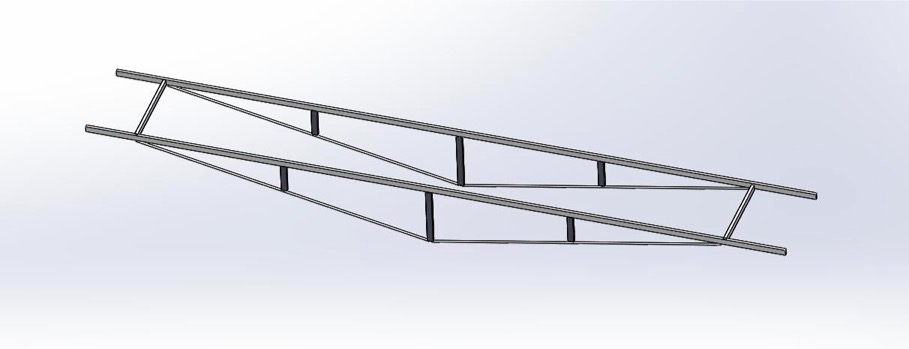
\includegraphics[width=15cm]{figure/designOverview/p3}
\end{center}
\end{figure}


\subsection{Cart}

The cart has ten main parts to fulfill the requirements: base, servo, wheel,
motor, battery, Arduino Board, Motor Driver and voltage transformer.

\bigskip
\noindent
\textbf{Base: Carbon Fibre} \\
\indent
Although we considered using Acrylic board, the fact that it is too thick, too
heavy and easy to break make us decide to use carbon fibre.
Carbon fibre is much lighter and stronger.
It also has a better looking. 

\bigskip
\noindent
\textbf{Servo: MG996R}  \\
\indent
We decided to use servo instead of motor to lift water because servo is more
powerful and easy to assemble. 
The first type we used is P0090.
It was not powerful enough, so we finally choose MG996R. 

\bigskip
\noindent
\textbf{Wheel: 3D-printed Plastic Wheel } \\
\indent
In order to fit the bridge, and meanwhile lower the influence to other parts of
the cart, we decided to print our own wheels in 3D.
The specially made wheels match the bridge well and guide the cart’s direction.

\begin{figure}[H]
\begin{center}
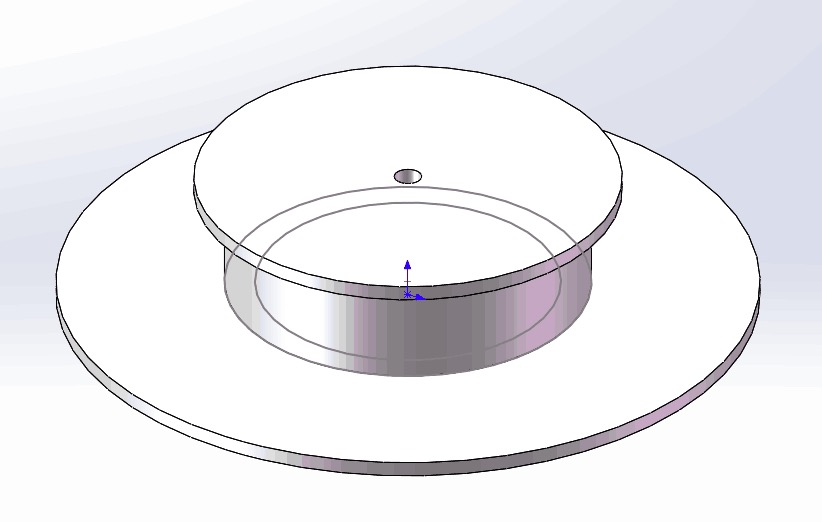
\includegraphics[height=4cm]{figure/designOverview/p2}
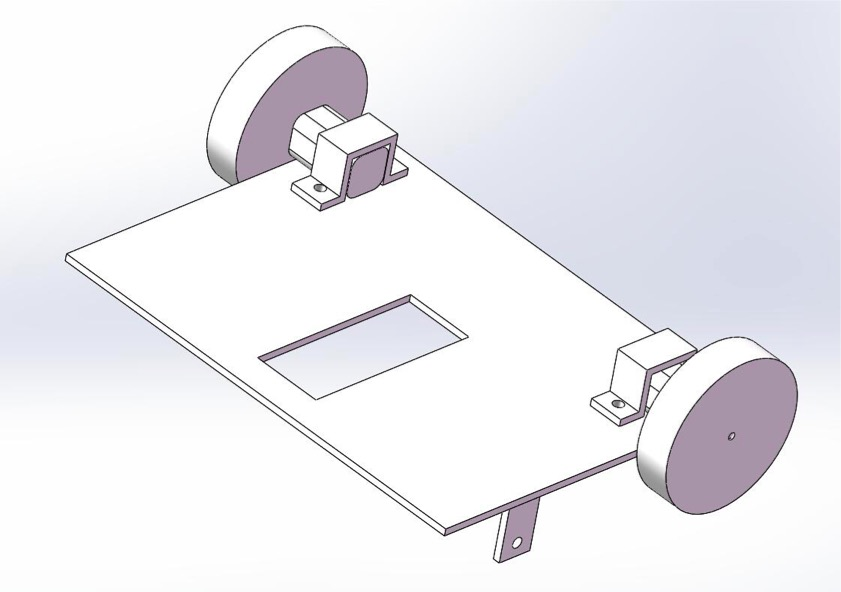
\includegraphics[height=4cm]{figure/designOverview/p1}
\end{center}
%\caption{Carbon fibre board \label{fig:carbonFiberBoard}}
\end{figure}

\bigskip
\noindent
\textbf{Motor: Gear motor N20 } \\
\indent
At first, we believe the high speed motor like 130 and 180 would give our cart
extraordinary speed.
But they were not powerful enough to move the cart on the bridge.
Also, the high speed motor has difficulty while stopping.
So we finally choose N20 gear motor.
It becomes slower but more powerful and stable.
In addition, N20 is also lighter than any high speed motor.  \\

\bigskip
\noindent
\textbf{Battery: 11.1V Battery } \\
\indent
The battery we chose has voltage 11.1V, which can well charge the Arduino board,
the motor board and the servo.
We choose 11.1V because we can have more choices of voltage using transformer.
We can adjust the speed of motor and servo easily.  

\bigskip
\noindent
\textbf{Arduino Board: UNO } \\
\indent
We first used Arduino UNO which was very light and small; however, we found it
too unreliable and not proper enough to be assemble on the cart, so we changed
to Arduino UNO.
It can provide all the functions we need stalely with a little weight increase.

\bigskip
\noindent
\textbf{Motor Driver: Motor Driver L9110 } \\
\indent
We first used Motor Driver L298n, which was provided by our project instructor;
however, we found the cooling n too heavy and to a certain degree useless for
our low-power cart, so we changed to Motor Driver L9110.

\bigskip
\noindent
\textbf{Voltage transformer:} \\
\indent
First, we did not use transformer to power the servo but Arduino board.
It takes more than 5 seconds to pull up the water.
After taking some calculation, the increase in voltage will shorten the time to
70\%.
So we finally applied transformer and lower the 11.1V from battery to 7.4V to
power the servo.

\subsection{Overall}

The bridge crane is a highly unified system composed of cart and bridge. Both the transport cart and the bearing structure take important roles in the whole system’s successful functioning.
In view of the cart’s performance after lifting water, we attached the top of paper stripe to the starting point of the car in order to disperse the force caused by the great acceleration. In view of the surface smoothness, we adapted gear motors to increase torque.
To enable the bridge to bear the cart which is much heavier than bridge itself, we adapted the beam with length-to-width ratio of two. Accordingly, we printed two special wheels to limit the track on the narrow deck. To enable the cart lift the bottle unimpededly, no stripe is supposed to attaching between the beams. Accordingly, we added four paper pillars to each beam’s bottom to keep them from rolling inwards or outwards. 
The diagram of the whole system is shown as below

\begin{figure}[H]
\begin{center}
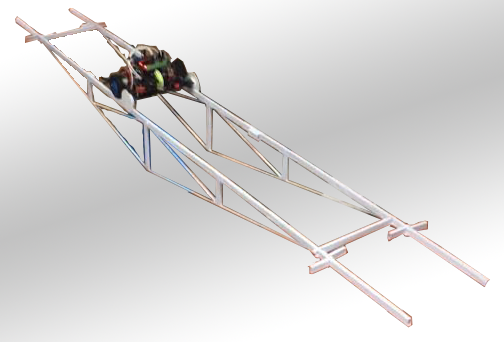
\includegraphics[height=6cm]{figure/designOverview/overallll}
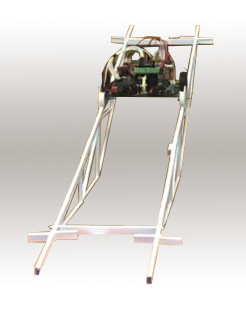
\includegraphics[height=6cm]{figure/designOverview/overallb}
\end{center}
\end{figure}

The components work well together. The strips spread out the pressure and the pillars help the cart control the direction. The whole system performs well in the cooperation.
		